
\usepackage[utf8]{inputenc}
\usepackage[round]{natbib}
\usepackage{graphicx}
\usepackage{tikz}
\usetikzlibrary{positioning}
\usepackage{tikz}

\pgfdeclareimage[width=\paperwidth]{mybackground}{poolModels.jpg}

\setbeamertemplate{title page}{

        \begin{picture}(0,0)

            \put(-30,-163){%
                \pgfuseimage{mybackground}
            }

            %\put(0,-110.7){%
            \put(-20,-220.7){%
                \begin{minipage}[b][55mm][t]{40mm}
                    \usebeamerfont{title}{\inserttitle\par}
                \end{minipage}
            }

            \put(230,-220.7){%
                \begin{minipage}[b][55mm][t]{40mm}
                    \usebeamerfont{title}{\insertsubtitle\par}
                \end{minipage}
            }
            \end{picture}

    }

\newcommand{\X}{\mathbf{X}}
\newcommand{\I}{\mathbf{I}}
%Information to be included in the title page:
\title{\bf \color{red} Pool models}
\subtitle{\bf \color{red} and attraction}
%\titlegraphic{
%	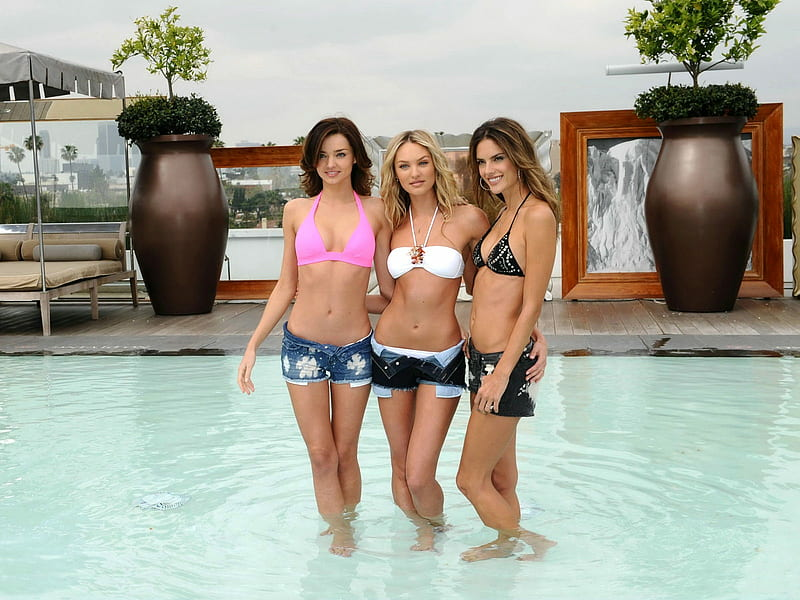
\includegraphics[width=\textwidth]{poolModels.png}
%}
%\author{Markus Müller}
%\institute{Overleaf}
%\date{11-16-2021}
\begin{document}
\begin{frame}
\titlepage
\end{frame}

\begin{frame}
\frametitle{Overview}
\tableofcontents
\end{frame}
\section{Attractors of autonomous systems}
\subsection{Frozen pool models and the role of $\X_c$}
\begin{frame}
  \frametitle{}
\end{frame}

\begin{frame}
\frametitle{Who is attracted to $\X_c$?}

\includegraphics[
  %width=\textwidth
  height=.1\textheight
]{Elsa.png}

$X_c(t)$ is the fixpoint of the system frozen at time $t$.
\[
\tilde{\X}^{\prime} = I_t - M_t \tilde{\X}
\]
with constant $M_t$ and $\I_t$  obtained
when we fix $M(t)$ and $\I(t)$ at the same time when we compute $\X_c(t)=M^{-1}(t)\I(t)$.
%\note{
%	\begin{enumerate}
%	\end{enumerate}
%}
\end{frame}

\section{Attractors for {\color{red}Non}autonomous Systems}
\subsection{Forward Attractors}
\begin{frame}
  \frametitle{\alert{Many} Forward attractors}
\end{frame}

\subsection{Pullback Attractor}
\begin{frame}
  \frametitle{\alert{unique} Pullback attractors}
  \[
    \nu(t):=\int_{-\infty}^t \Phi(t,u) \I(u) du \quad \text{for all} t \in T
  \]
  \[
    \lim_{t_0 \rightarrow -\infty} dist(\phi(t,t_0,B),{\nu(t)})=0 \quad \text{for all} t \in T
  \]
\end{frame}

\begin{frame}
  \frametitle{}
	\begin{thebibliography}{}
	\bibitem[Metzler, Müller, Sierra, 2018]{Metzler2018PNAS}
	Metzler, H., M{\"u}ller, M., and Sierra, C. (2018).
	\newblock Transit-time and age distributions for nonlinear time-dependent
	  compartmental systems.
	\newblock {\em Proceedings of the National Academy of Sciences}, 115:201705296.
	\end{thebibliography}
\end{frame}

\end{document}
